\documentclass[12pt, a4paper]{scrartcl}
\usepackage[utf8]{inputenc}
\usepackage[T1]{fontenc}
\usepackage[ngerman]{babel}
\usepackage{SIunits}
\usepackage{csvsimple}
\usepackage{graphicx}
\usepackage{amsmath}
\usepackage{enumitem}
\usepackage{float}
\usepackage{verbatim} %für Kommentare
\usepackage{listings} %Zur Code-Einfügung
 \usepackage{subfigure}  %Bilder nebeneinander darstellbar

\usepackage[
colorlinks,
pdfpagelabels,
bookmarksopen = true,
bookmarksnumbered = true,
linkcolor = black,
plainpages = false,
hypertexnames = false,
citecolor = black
]{hyperref}

%\usepackage{biblatex}
%\addbibresource{Dateien/bibliography.bib}

%\usepackage{titlesec}
%\titleformat{name=\section,numberless}{}
%Entfernt Zahlen vor Kapitelüberschriften
%\titleformat{\chapter}[display]{\normalfont\bfseries}{}{0pt}{\Huge}

\usepackage[subfigure]{tocloft}
%Punktlinie auch nach Kapiteln im Inhaltsverzeichnis
\renewcommand{\cftsecleader}{\cftdotfill{\cftdotsep}}

%Zeilenabstände
\renewcommand{\baselinestretch}{1.5} 

\usepackage{geometry}
%Rand-Abstände
\geometry{verbose, left=20mm, right=20mm, top=30mm, bottom=30mm}

%\usepackage{titlesec}
%\titleformat
%{\chapter} % command
%[hang] % shape
%{\bfseries\Huge} % format
%{\thechapter} % label
%{0.5ex} % sep
%{} % before-code
%[] % after-code


% Für Grafiken
\usepackage{tikz}
\usepackage{pgfplots}
\usetikzlibrary{datavisualization}
\usetikzlibrary{datavisualization.formats.functions}


%%%%%%%%%%%%%%%%%%% Aufteilung: %%%%%%%%%%%%%%%%%%%
% Lea:
%Abstandserkennung
%(GeogebraDatei im doc Ordner)

% Adrian:
%Motoransteuerung
%Umgebung (Räumliche Umgebung des Autos mit Bildern. Auch aus der Sicht des Autos)

% Julian W.:
%Softwareplattform
%Interprozesskommunikation

% Julian F.
%Linienerkennung
%Zielsetzung

% René
%Hardwareplattform
%Einleitung
%Struktur

% Gemeinsam:
%Komplikation und Fehler
%Auswertung


\begin{document}

%%%%%%%%%%%%%%%%%%% STARTSEITE %%%%%%%%%%%%%%%%%%%

\begin{center}
	
	\begin{figure}[H]
		\centering
		
\includegraphics[width=10cm]{Bilder/fh-wedel-logo.png}
	\end{figure}

	\vspace*{1.5cm}
	\Large{\textbf{ R O B O T I K\quad P R A K T I K U M \\ Wintersemester 2017/ 2018\\}}
	\vspace*{1.5cm}
	\huge{\textbf{Dokumentation - Gruppe 1\\}}
	\vspace*{1.5cm}
	
	\vfill
	\begin{table}[h]\centering
		\begin{tabular}{l l}
			 &  tinf101030 - Julian Finck \\
			 & \\
			 & tinf101364 - René P. Keller  \\
			 & \\
			 & inf101301 - Lea Morschel \\
			 & \\
			 & tinf101313 - Adrian Sorge \\
			 & \\
			 & tinf101087 - Julian Weihe \\
		\end{tabular}
	\end{table}

\end{center}


\newpage
\tableofcontents % generiertes Inhaltsverzeichnis
\newpage


%%%%%%%%%%%%%%%%%%% INHALTE %%%%%%%%%%%%%%%%%%%

%%% Neues Kapitel %%%
\section{Einführung}

Das Robotik-Praktikum, wessen Ergebnis diese Dokumentation festhält, fand parallel zur und in Kombination mit der Bachelor-Vorlesung 'Einführung in die Robotik' statt, welche von Herrn Prof. Dr. Ulrich Hoffmann im Wintersemester 2017 gehalten wurde.

Ziel war die Vertiefung und Anwendung der in der Vorlesung vermittelten Inhalte, wobei der diessemestrige Schwerpunkt  auf autonomen Robotern lag. Im Praktikum wurde mit einem AADC\footnote{Audi Autonomous Driving Cup\cite{aadc-website}} 2017 Audi-Modell im Maßstab 1:8 gearbeitet. Es sollte zu Beginn eine nicht näher eingeschränkte Zielsetzung ausgearbeitet werden, welche auf der grundlegenden Anforderung der kollisionsfreien Fahrt aufbauen sollte.

%%% Neues Kapitel %%%
\subsection{Zielsetzung} \label{zielsetzung}

Im Kontext der gegebenen Grundanforderung der Kollisionsvermeidung wurden eigene Ziele definiert. Das Auto sollte später in der Lage sein, einer zentralen blauen Fahrbahnmarkierung zu folgen, dies unter verschiedenen Lichtverhältnissen. Bei Näherkommen eines von Ultraschallsensoren detektierbaren Hindernisses soll das Modell langsamer werden und vor ihm zum Stehen kommen sowie die Fahrt erst wieder aufnehmen, wenn die Sensoren signalisieren, dass die Fahrbahn wieder frei ist.

Die zu Beginn des Praktikums ausgearbeitete Roadmap findet sich in Abbildung \ref{img:Roadmap_Gr1}.
\newpage
Die Umsetzung des Projektes wurde zu Anfang in vier Bereiche unterteilt:
\begin{enumerate}
		\item{Linienerkennung und -verwertung
		\begin{enumerate}
			\item Mittelpunktbestimmung
			\item Testen unter verschiedenen Lichtintensitäten
	\end{enumerate}}
	\item{Abstandserkennung und Kollisionsvermeidung
	\begin{enumerate}
		\item Messwertverarbeitung der Ultraschallsensoren
		\item Messwertglättung durch Filterung (Kalman)
	\end{enumerate}}
	\item {Motorsteuerung
		\begin{enumerate}
		\item Schnittstellendefinition zur Ansteuerung
		\item Steuerung von Geschwindigkeit und Lenkung
		\end{enumerate}}
		\item{Zusammenbringung/ Fusionsschnittstelle
		\begin{enumerate}
			\item Definition und Ausarbeitung des Controllers (Verhaltens-Logik)
			\item Problembehandlung, Feinabstimmung, Testung
		\end{enumerate}}
\end{enumerate}

\begin{figure}
\centering
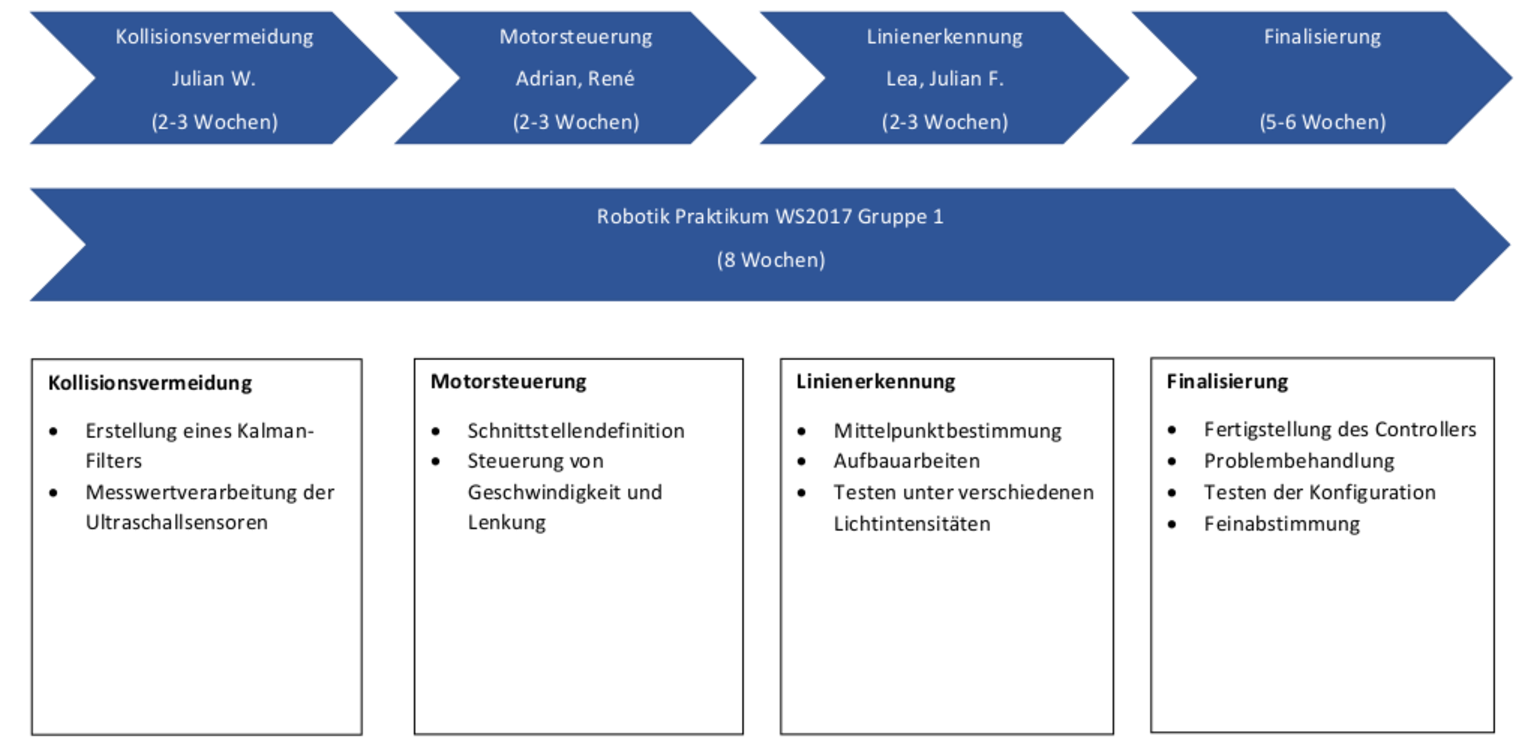
\includegraphics[width=\textwidth, height=9cm, keepaspectratio]{Bilder/Roadmap_Gr1.pdf}
\caption{Zu Projektbeginn erstellte Roadmap}
\label{img:Roadmap_Gr1}
\end{figure}


\newpage
%%% Neues Kapitel %%%
\section{Grundlagen}
Im Folgenden werden die Grundlagen, bestehend aus Aufbau des genutzten Modellautos, der darauf laufenden Software, sowie das genutzte Framework erläutert, welche für das Verständnis des Projektes essenziell sind.

\subsection{Hardwareplattform}
Das Audimodell bietet verschiedene Hardwarekomponenten, um das autonome Fahren zu verwirklichen.

TODO: Bild vom Audi gesamt

\subsubsection{Grundkomponenten}
Die Stromversorgung während der Fahrt wird durch zwei Akkus sichergestellt.

\subsubsection{Rechner}
Herzstück des Audi ist das \emph{GIGABYTE GA-Z170N-WIFI miniITX} Mainboard mit einem \emph{Intel Core i3-6100T} und 8 GB DDR4 RAM. Unterstützt wird es von einer \emph{NVIDIA GeForce GTX 1050Ti}. 

Das Betriebssystem wird von einem USB-Stick gebootet, um das Auto mit mehreren Gruppen nutzen zu können.
TODO: Bild vom Audi, vor allem mit der Intel

\subsubsection{Aktoren}
Angetrieben wird das Modell von vier \emph{Hacker SKALAR 10 21.5 Brushless Motor 1/10}.
Die Lenkung funktioniert über \emph{Absima 'ACS1615SG' Combat Series} Servos. 

\subsubsection{Sensoren}
Die Linienerkennung arbeitet mit der Intelkamera, die mit einer anderen Position und einem anderen Winkel benutzt wird, als im Basismodell. Zum Vergleich siehe Abbild 1 und 2. Grund ist der verbesserte Blick auf den Nahbereich und das mittig ausgerichtete Bild.

TODO: Bild von den Sensoren und Arduinos

\begin{figure}[ht]
	\centering
	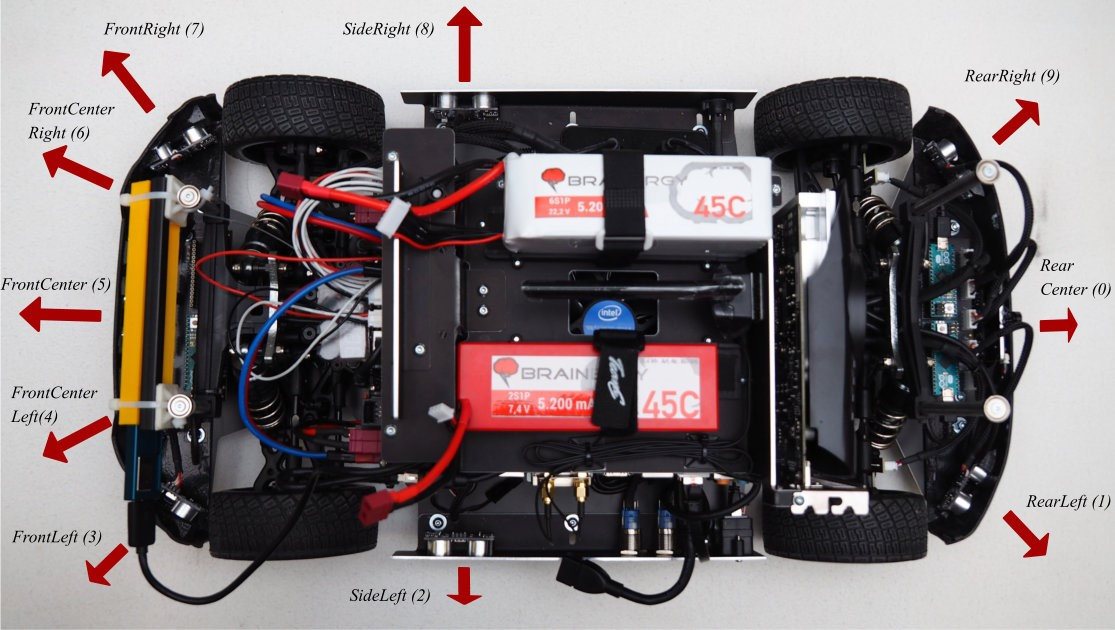
\includegraphics[width=\textwidth, height=10cm, keepaspectratio]{Bilder/car_sensors.jpg}
	\caption{Platzierung der Ultraschallsensoren am Audi-Modell}
	\label{img:car_ussensors}
\end{figure}

\begin{comment}
\begin{figure}[ht]
	\centering
	\begin{tikzpicture}[xscale=0.05,yscale=0.05]
	
	%Auto-Umriss
	\draw[line width=0.2mm] (-20,20) -- (-10,0) -- (10,-10) -- (40,-10) -- (60,0) -- (70,20); %Hinterseite
	\draw[line width=0.2mm] (-20,120) -- (-20,20);	%linke Seite
	\draw[line width=0.2mm] (70,20) -- (70,120);	%rechte Seite
	\draw[line width=0.2mm] (-20,120) -- (-10,140) -- (10,150) -- (40,150) -- (60,140) -- (70,120); %Vorderseite
	
	\draw[line width=0.2mm, ->] (25,50) -- (25,100); %Mittelpfeil
	
	%Pfeile und Beschriftungen der Sensor-Lagen
	\draw[->] (50,0) -- (60,-15) node[below right]{$Rear Right(9)$};
	\draw[->] (65,70)-- (80,70) node[right]{$Side Right(8)$};
	\draw[->] (60,130) -- (80,140)  node[above right] {$Front Right(7)$};
	\draw[->] (45,140) -- (65,160)  node[above right] {$Front Center Right(6)$};
	\draw[->] (25,145) -- (25,170) node[above] {$Front Center(5)$};
	\draw[->] (5,140) -- (-15,160)  node[above left] {$Front Center Left(4)$};
	\draw[->] (-10,130) -- (-30,140)  node[above left] {$Front Left(3)$};
	\draw[->] (-15,70) -- (-30,70) node[left]{$Side Left(2)$};
	\draw[->] (0,0) -- (-10,-15) node[below left]{$Rear Left(1)$};
	\draw[->] (25,-5) -- (25,-20) node[below]{$Rear Center(0)$};
	
	\end{tikzpicture}
	\caption{Platzierung der Ultraschallsensoren am schematischen Modell}
	\label{graph:us-car}
\end{figure}
\end{comment}

Zur Kollisionsvermeidung werden die verbauten Ultrasonic Sensoren verwendet (siehe \autoref{img:car_ussensors}). Ansteuern lassen sich diese über Arduinos, die mit dem Mainboard verbunden sind. Der Audi besitzt insgesamt zehn Stück, von denen fünf, in unterschiedlichen Winkeln, nach vorne, jeweils einer zu jeder Seite und drei, wieder in unterschiedlichen Winkeln, nach hinten ausgerichtet sind. Die drei hinteren Sensoren bekommen nicht so viel Gewichtung, da das Auto in unserem Projekt nicht rückwärts fahren soll.


\subsection{Softwareplattform}
Das Modellauto verwendet die Ubuntu Version 16.04 und zur Bildschirmübertragung ist der x11vcn Serverdienst eingerichtet. Die Software EB Assist ADTF 2.14 von Elektrobit ist installiert, um die damit bereitgestellte Programmoberfläche und das ADTF-Framework\footnote{Automotive Data and Time-Triggered Framework\cite{adtf-website}} zu verwenden.

\subsubsection{ADTF-Framework: Grundlegende Strukturen}
 Das Framework stellt Funktionen zur Kommunikation mit den im Abschnitt 'Hardwareplattform' erläuterten Sensoren und Kameras bereit. Außerdem ermöglicht es eine Programmaufteilung in Funktionsblöcke, \emph{Filter} genannt, welche parallel auf mehreren Prozessorkernen ausgeführt werden können. Die Kommunikation zwischen diesen Blöcken wird über Nachrichtenqueues und Priorisierung vom Framework sichergestellt. Die Ausführung der Funktionsblöcke wird einstellbar periodisch eventgesteuert ausgelöst und beginnt meist mit dem Anstoß zum Auslesen der Sensoren, welche dann das Event über die Queues an andere Funktionsblöcke weitergeben.

Von der Benutzeroberfläche aus lassen sich die Funktionsblöcke grafisch miteinander verbinden, welches die Kommunikation zwischen den Blöcken repräsentiert, und die Ausführung der Funktionen starten. Des Weiteren gewährt die Oberfläche Zugriff auf fertige Funktionsblöcke, etwa zum Anzeigen und Abspeichern von Kamerabildern und Sensordaten oder zum  Abspielen selbiger.
Durch Referenzen aus dem Programm heraus können über die Benutzeroberfläche bestimmte Parameter zur Initialisierung und zur Laufzeit gesetzt werden.


\newpage
%%% Neues Kapitel %%%
\section{Implementierung}

\subsection{Umgebung}

Die Zielsetzung sieht vor, das Auto eine blaue Linie verfolgen zu lassen. Zu Testzwecken wurde daher auf dem Boden eine große, ovalförmige Linienstruktur mit mattblauem Klebeband befestigt, deren Maße etwa 1,5 m x 3 m beträgt. Zur Vermeidung von störender Spiegelung wurde zudem das Fenster zugestellt, um die Sonneneinstrahlung zu minimieren.

TODO: Bild(er) der Umgebung

\subsection{Projektumsetzung}

Das Projekt wurde zu Beginn in verschiedene Aufgabenbereiche aufgeteilt, die separat bearbeitet wurden (siehe \autoref{zielsetzung}). Die vier großen Bereiche sind im Folgenden näher beschrieben.

\begin{enumerate}
	\item Linienerkennung und -verfolgung
	\item Abstandserkennung und -verwertung
	\item Motorsteuerung
	\item Fusionsschnittstelle
\end{enumerate}


\subsubsection{Linienerkennung und -verfolgung}
Damit das Auto der blauen Fahrbahnlinie folgen kann, wird die Linie im Kamerabild detektiert. Anschließend wird die Position der Linie ausgewertet, um daraus Steuersignale für die Lenkung zu gewinnen. Diese Aufgaben werden von zwei Filtern gelöst:

\paragraph{BlueImgFilter}
\begin{figure}[h]
	\centering
	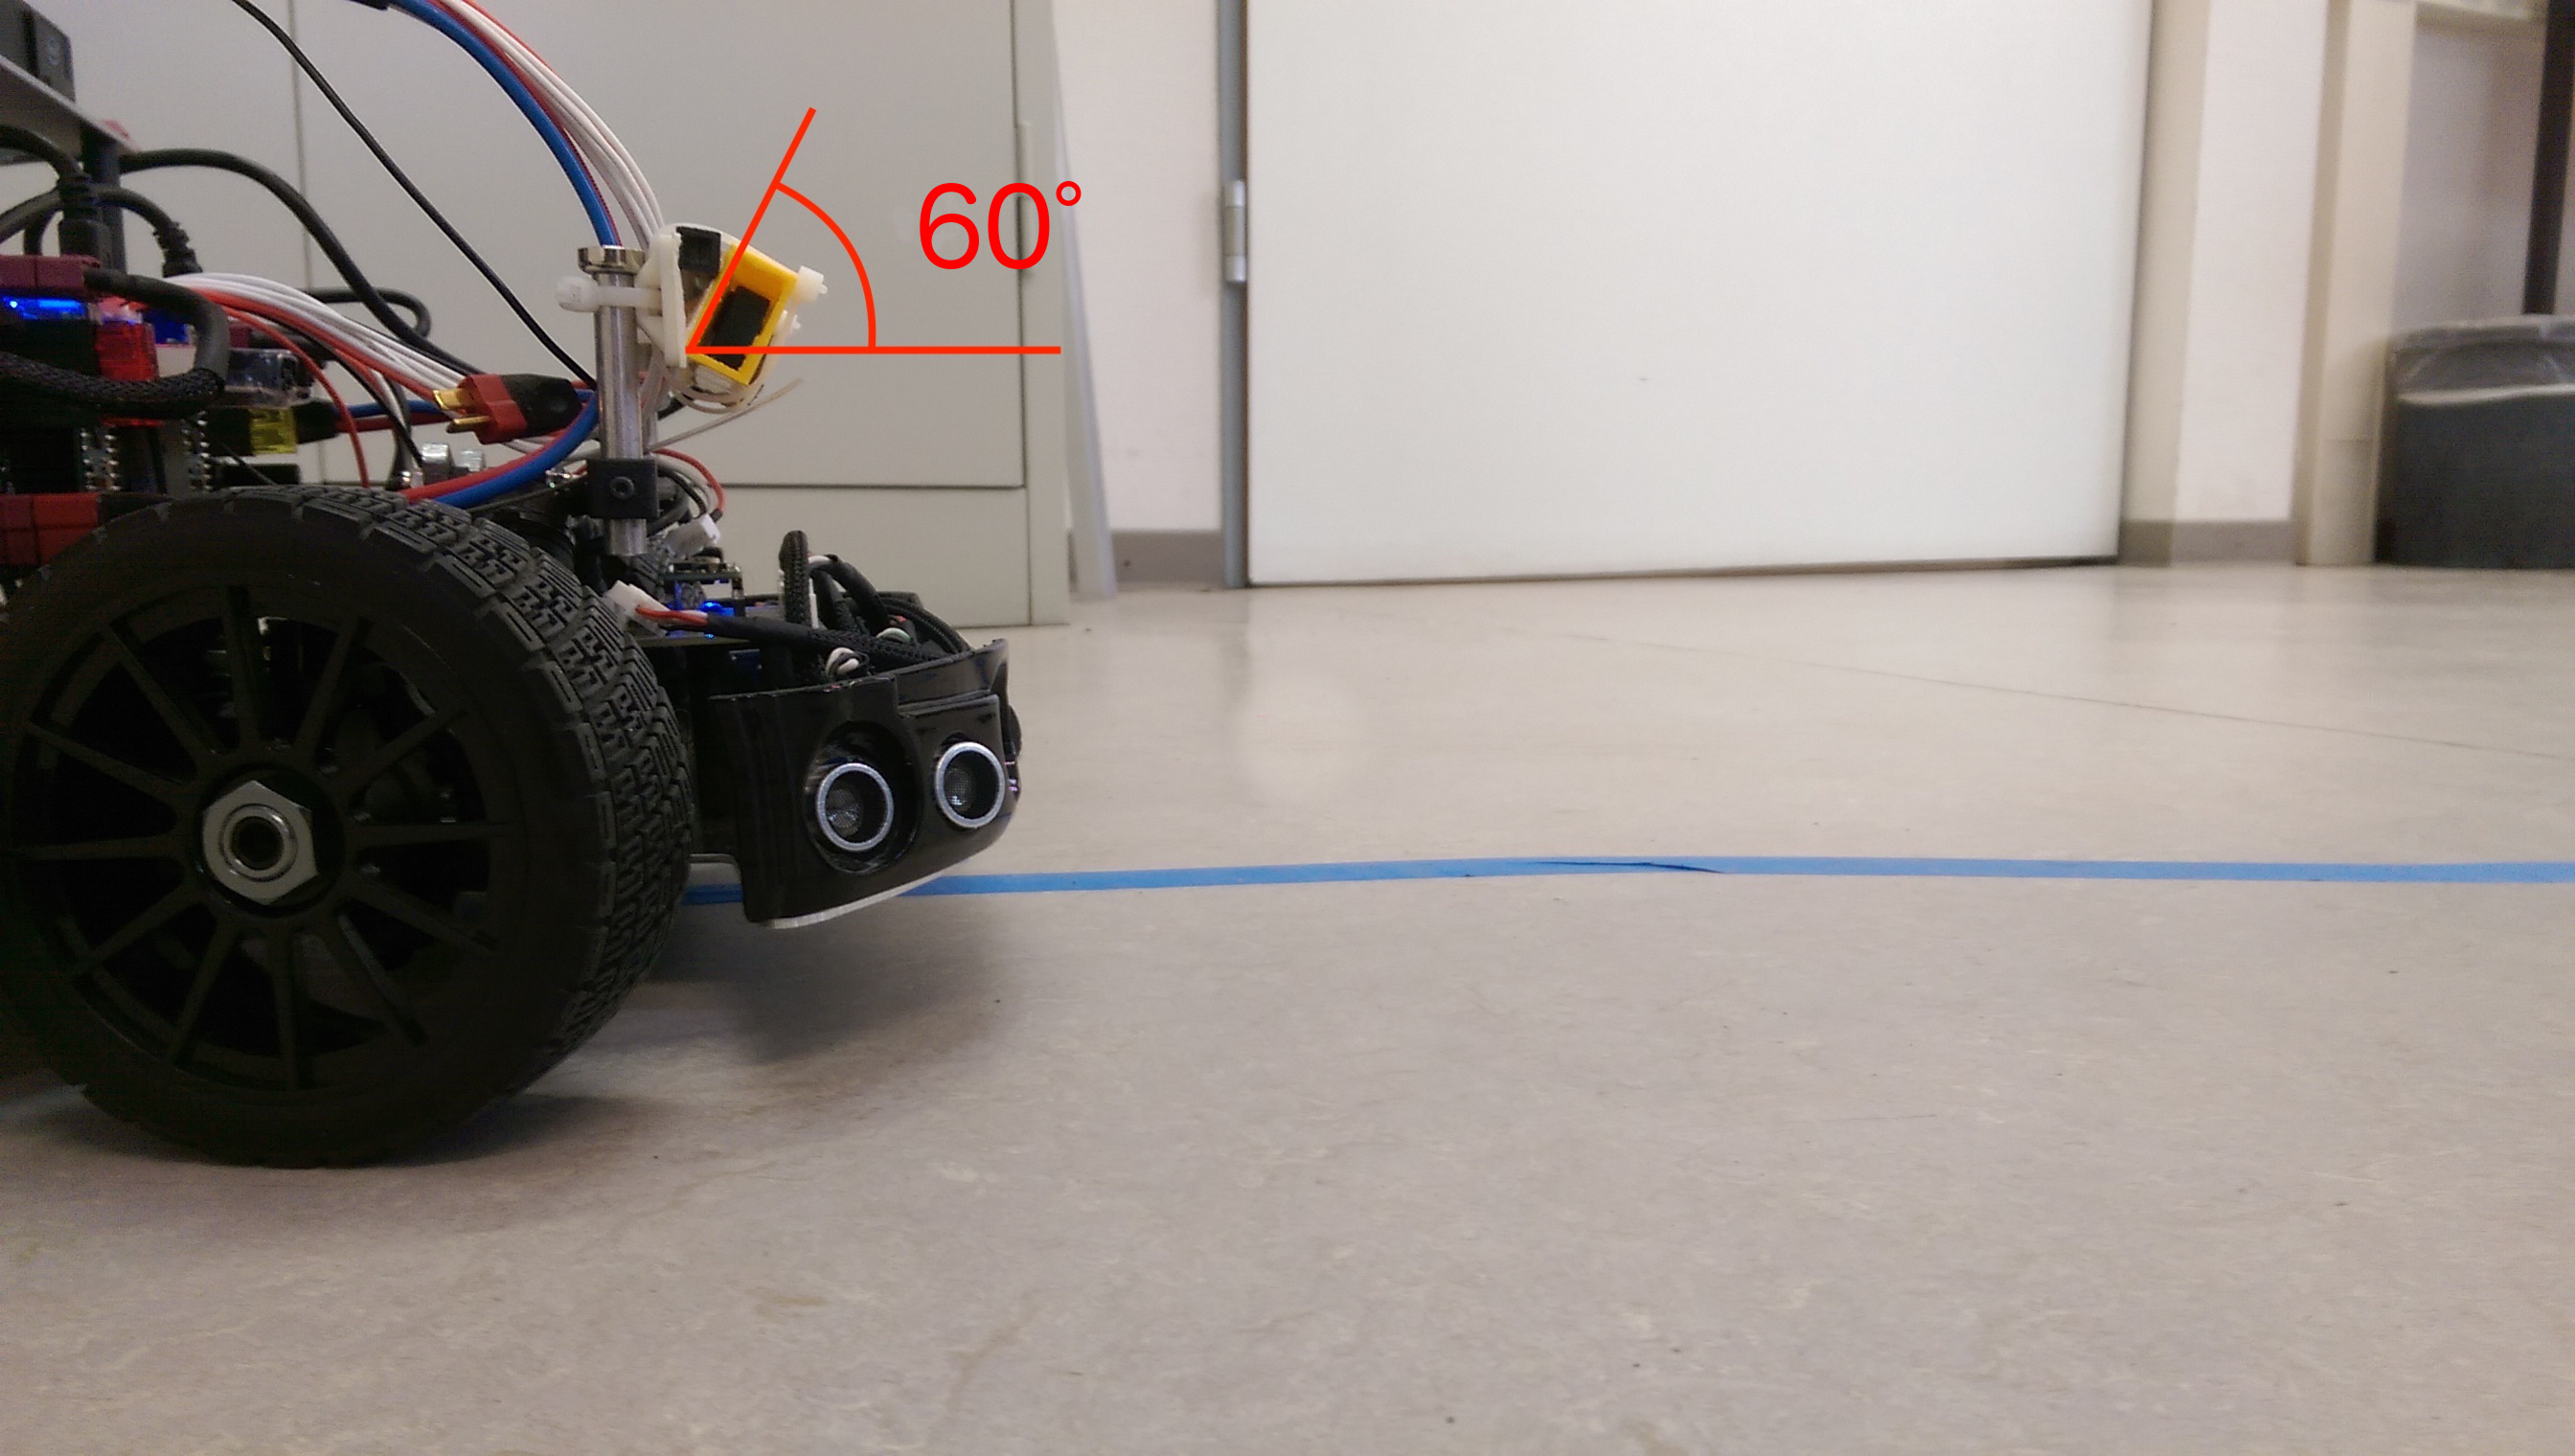
\includegraphics[width=\textwidth, height=7cm, keepaspectratio]{Bilder/carCameraFrontAngle60.jpg}
	\caption{Winkel der Frontkamera am Modell}
	\label{img:carCameraFrontAngle60}
\end{figure}

Dieser Filter markiert die Fahrbahnlinie und greift dafür auf die OpenCV Bibliothek zurück. Die Kamera ist in einem 60 Grad Winkel montiert (Siehe Abbildung 1). Es ist davon auszugehen, dass die Fahrbahnlinie der einzig blaue Bildinhalt im relevanten Bildausschnitt ist. Zunächst wird das Eingangsbild mit OpenCV vom RGB- in den HSV-Farbraum transformiert, um die Festlegung von Ober- und Untergrenzen für Blauwerte zu vereinfachen. Mittels der OpenCV-Funktion \emph{inRange()} werden anschließend alle nicht blauen Bildinhalte herausgefiltert und ein Binärbild zurückgegeben, welches alle blauen Flächen markiert. Die endgültigen Farbwertgrenzen sind das Ergebnis von folgenden Versuchen mit variierenden Lichtverhältnissen:

\begin{description}
	\item[Versuch 1 - Szenario mit geringster Lichtintensität]
	Lichtverhältnisse:	Jalousie runtergelassen, Beleuchtung aus, Tageslicht von den Oberlichtern, bewölkt (mittags)
	\item[Versuch 2 - Szenario mit höchster Lichtintensität]
	Lichtverhältnisse:	Jalousie oben, alle Lichter an, keine Wolken (mittags) 
\end{description}

Auswertung:

Als Ergebnis dieser Versuche sind die in \autoref{tbl:linedet_lighttest} folgenden Unter- bzw. Obergrenzen der Funktion \emph{inRange()} eruiert worden, welche in beiden Extremfällen eine Positionsberechnung der Linie ermöglichen.

\begin{table}[h]
	\caption{Ergebnisse der Tests bei verschiedener Lichtintensität}
	\centering
	\begin{tabular}{ c | c | c |}
		& Untergrenze & Obergrenze \\ \hline
		Hue & 95 & 130 \\ \hline
		Saturation & 100 & 255 \\ \hline
		Value & 70 & 255 \\
	\end{tabular}
	\label{tbl:linedet_lighttest}
\end{table}

Im dunklen Szenario beeinträchtigt der geringe Rauschabstand die Erkennung der Linie leicht, wie in \autoref{img:line_filt_viel_u_wenig_licht} (a) zu erkennen ist. Die Ergebnisse lassen dennoch eine ausreichend robuste Positionsberechnung zu.

Im normal-hellen Szenario ist der Rauschabstand so groß, dass \emph{inRange()} die Fahrbahnmarkierung nahezu optimal ausschneidet (\autoref{img:line_filt_normal_u_kurve} (a)). Reflexionen der Sonne können zu Clipping führen und verhindern eine durchgehende Erkennung der Markierung (siehe \autoref{img:line_filt_viel_u_wenig_licht} (b)).

\begin{figure}[h]
	\subfigure[Viel Licht und Reflektion]{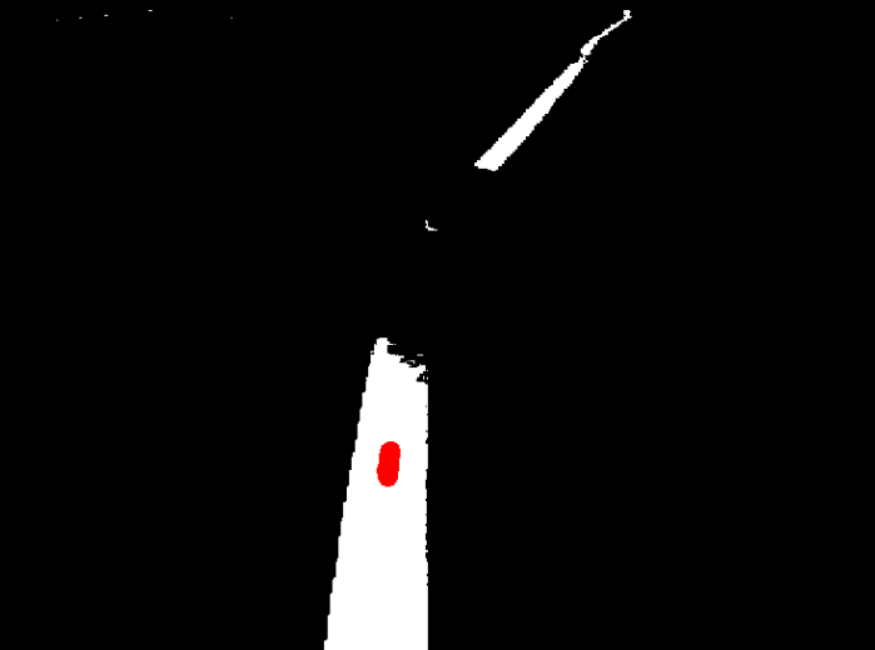
\includegraphics[width=0.49\textwidth]{Bilder/line_filt_vielLicht_reflektion.png}}
	\subfigure[Wenig Licht]{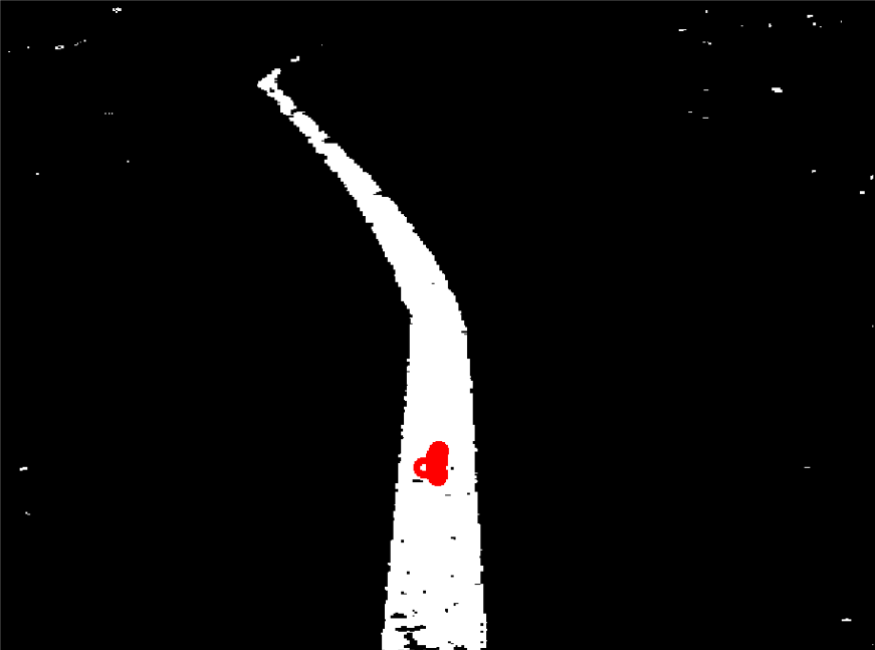
\includegraphics[width=0.49\textwidth]{Bilder/line_filt_wenigLicht.png}}
	\caption{Gefilterte Linienerkennung unter extremen Lichtverhältnissen}
	\label{img:line_filt_viel_u_wenig_licht}
\end{figure}

Daher ist es wichtig, direkte Sonneneinstrahlung auf der Fahrbahn zu vermeiden.  

\begin{comment}
	\begin{figure}[h]
	\centering
	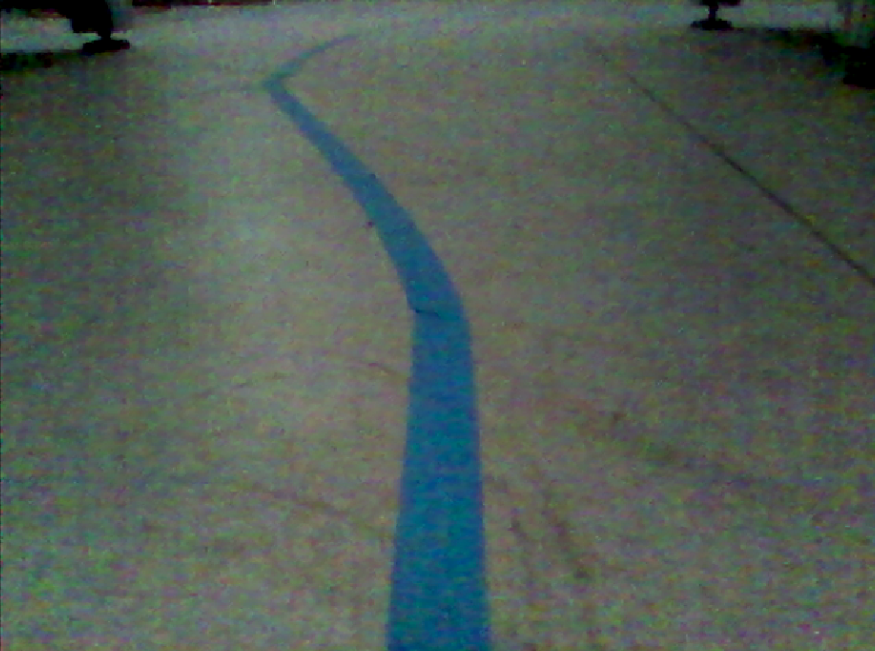
\includegraphics[width=\textwidth, height=7cm, keepaspectratio]{Bilder/line_unfilt_wenigLicht.png}
	\caption{Ungefilterte Aufnahme der Fahrlinie bei wenig Licht}
	\label{img:line_unfilt_wenigLicht}
	\end{figure}
\end{comment}


\paragraph{OneLineDetect}
Dieser Filter erhält das Binärbild und ermittelt die Position der blauen Linie relativ zur Position des Autos. Dafür wird in einer Bildzeile kurz unterhalb der Bildmitte (korreliert mit dem Bereich 20 cm vor dem Auto) nach der größten Anzahl weißer, zusammenhängender Pixel gesucht. Der Mittelpunkt wird berechnet und als Zentrum der dort verlaufenden Linie interpretiert. Der Abstand zwischen ermittelten Linienmittelpunkt und Bildmitte wird auf einen Wert zwischen -100 und 100 normiert und ausgegeben (siehe \autoref{graph:oneLineDet_reldotpos}).

\begin{figure}[h]
	\centering
	\begin{tikzpicture}[xscale=0.05,yscale=0.05]
	\draw[-] (-100,0) -- (100,0) node[right] {$Bildbreite$};
	\foreach \i in {-100, 0, 100}{
		\draw[-] (\i,-2) -- ( \i,2) node[above] {$\i$};
	}
	\draw[line width=1mm] (10,-2) -- (10,2) node[above right] {Bsp. Erkannte Linie};
	\end{tikzpicture}
	\caption{Beispiel eines Linienmittelpunktes (10) innerhalb eines Bildes, normiert auf den Bereich -100 bis 100}
	\label{graph:oneLineDet_reldotpos}
\end{figure}

Um die Berechnung der Linienmitte robuster zu gestalten, was besonders bei verrauschten Kamerabildern in dunklen Lichtverhältnissen nützlich ist, wird die Linienmitte auch in benachbarten Bildzeilen berechnet. Auf die errechneten Linienmittelpunkte wird der Median-Filter angewendet. Außerdem gibt es eine Mindestanzahl an zusammenhängenden weißen Pixeln, die erreicht werden muss, um als Fahrbahnmarkierung zu gelten.

Wird beispielsweise in einer Kurve in dem Bereich unter der Bildmitte keine Linie detektiert, so wird in einem zweiten Suchbereich nahe des unteren Bildrandes gesucht (siehe \autoref{img:line_filt_normal_u_kurve} (b)). Dieser Bereich korreliert mit dem Abstand von 5 cm vor dem Auto.

Wird auch hier keine Linie detektiert, wird der Wert -101 ausgegeben. 

Auf den Abbildungen \ref{img:line_filt_viel_u_wenig_licht} und \ref{img:line_filt_normal_u_kurve} sind in Rot jeweils diejenigen Punkte markiert, die zur Linienpositionierung erkannt wurden.


\begin{figure}
	\subfigure[Wenig gekrümmte Fahrstrecke]{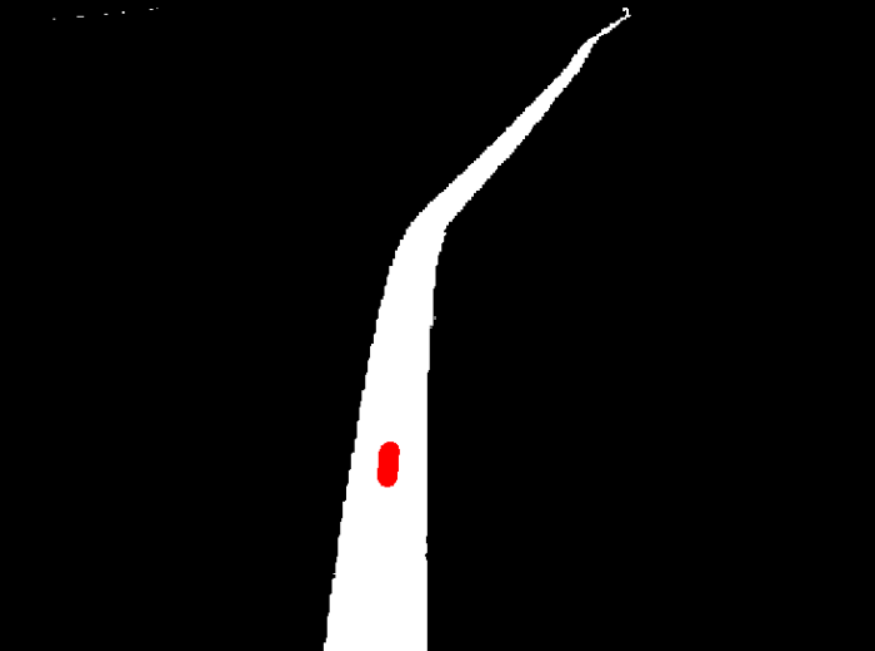
\includegraphics[width=0.49\textwidth]{Bilder/line_filt_normal.png}}
	\subfigure[Enge Kurve]{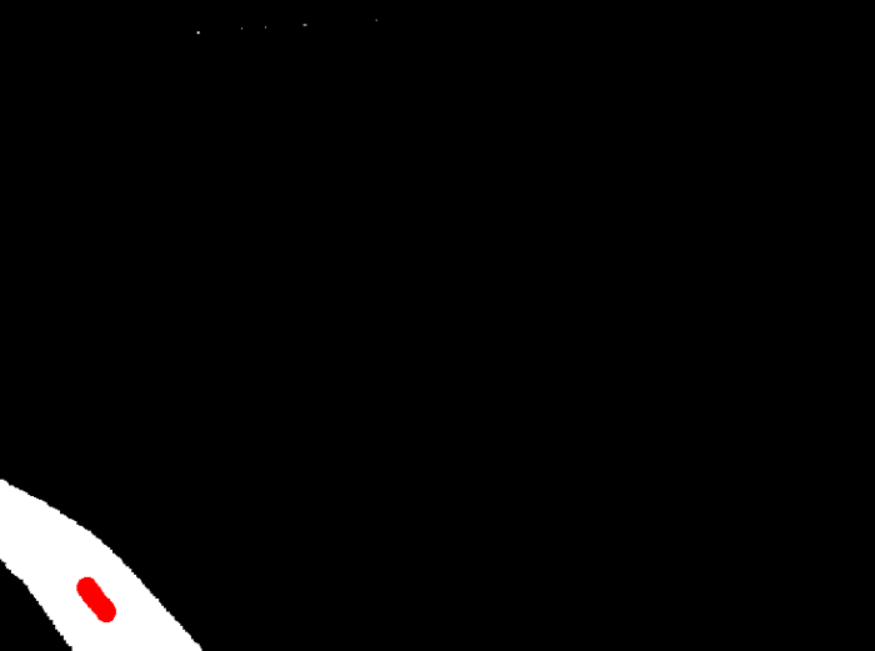
\includegraphics[width=0.49\textwidth]{Bilder/line_filt_engeKurve.png}}
	\caption{Gefilterte Linienerkennung unter normalen Lichtverhältnissen - unterschiedliche Behandlung gemäß Fahrbahnkrümmung}
	\label{img:line_filt_normal_u_kurve}
\end{figure}


\subsubsection{Abstandserkennung und -verwertung}
Die Abstandserskennung ist eine der grundlegenden Anforderungen an einen autonomen Roboter zur Ermöglichung von gefahrloser Navigation. In diesem Projekt wird sie auf Basis von Messwerten der zehn im Auto verbauten Ultraschallsensoren (siehe \autoref{img:car_ussensors})  implementiert.

Die eingehenden Abstandswerte liegen im Bereich von 0 bis 400 cm. Diese werden unterschiedlich gewichtet, dann der geringste Wert in eine Geschwindigkeit umgerechnet. Die Übersetzung eines Abstands- in einen Geschwindigkeitswert wird anhand einer linearen Funktion realisiert, die einen minimalen  Input-Grenzwert zum Anstoßen der Bewegung und gleichsam einen maximalen Input-Wert beinhaltet, ab dem die volle Geschwindigkeit zurück gegeben wird (siehe \autoref{graph:disttospeed}). Dies dient dazu, einen gewissen Mindestabstand beim Fahren nicht zu unterschreiten, sowie zum Ignorieren von Hindernissen, die weiter als ein gewisser Maximalwert von den Sensoren entfernt aufgefasst werden. Ersterer wurde durch Testergebnisse statisch auf 20 cm gesetzt, letzterer auf 100 cm. Im Abstands-Wertebereich von 20 cm bis 100 cm gilt die lineare Funktion \emph{y = x}.

\begin{figure}[ht]
	\centering
	\begin{tikzpicture}[xscale=0.05,yscale=0.05,domain=0.125:220,samples=400]
	\draw[->] (-10,-10) -- (180,-10) node[below] {$Abstand (\centi\meter)$}; %x-Achse
	\draw[->] (0,-20) -- (0,115) node[left] {$Geschwindigkeit (Prozent)$}; %y-Achse
	\foreach \i in {20,40,...,150} { %x-Achsen-Schritte
		\draw (\i,-9) -- (\i,-11) node[below] {$\i$};
	}
	\foreach \i in {0,20,...,100} { %y-Achsen-Schritte
		\draw (1,\i) -- (-1,\i) node[left] {$\i$};
	}
	\draw[blue] (0,0) -- (20,0) ;
	\draw[blue, dotted] (20,0) -- (20,20);
	\draw[blue] (20,20) -- (100,100) -- (140, 100);
	\end{tikzpicture}
	\caption{Übersetzung von Abstandswert in prozentuale Geschwindigkeit}
	\label{graph:disttospeed}
\end{figure}

Die Geschwindigkeit wird mithilfe des kleinsten von allen Ultraschallsensoren gemessenen Abstandswertes berechnet. Da den zur Seite oder gar nach hinten gerichteten Sensoren bei geradliniger Fahrt nicht die selbe Priorität beigemessen werden sollte, wie den nach vorne ausgerichteten, wo der Abstand eher kollisionsrelevant ist, wird zunächst jeder Wert nach Relevanz gewichtet und entsprechend zu einem neuen Wert verrechnet. Mit jedem Sensor wird ein Winkel assoziiert, welcher auf den Bereich zwischen -1 und 1 abgebildet wird, wobei 0 die frontale Ausrichtung beschreibt. Der Bereich von 0 bis -1 beschreibt im Modell den gegen den Uhrzeigersinn gerichteten Halbkreis bis zum nach hinten gerichteten Sensor (\autoref{img:car_ussensors}; der Reihe nach die Sensoren (5), (4), (3), (2), (1), (0)) und äquivalent der von 0 bis 1 gehende Bereich den Halbkreis im Uhrzeigersinn zum nach hinten gerichteten Sensor  (\autoref{img:car_ussensors}; der Reihe nach die Sensoren (5), (6), (7), (8), (9), (0)). Alle rückgerichteten Sensoren wurden der Einfachheit halber auf 1 respektive -1 abgebildet, da sie bei der normalen Fahrt nicht weiter von Interesse sind. Die Zuordnung der Winkel ist veranschaulicht in \autoref{img:car_ussensors}. 

\begin{figure}[ht]
	\centering
	\begin{tikzpicture}[xscale=3,yscale=3]
	\draw[->] (0,-1.1) -- (0,1.1);	%Pfeil
	
	%Zahlen auf dem Strahl
	\draw  (0.05,-1) -- (-0.05,-1) node[left] {$(-180\degree) -1$};
	\draw  (0.05,-0.7) -- (-0.05,-0.7) node[left] {$(-126\degree) -0.7$};
	\draw  (0.05,-0.4) -- (-0.05,-0.4) node[left] {$(-72\degree) -0.4$};
	\draw  (0.05,-0.2) -- (-0.05,-0.2) node[left] {$ (-36\degree) -0.2$};
	\draw  (0.05,-0) -- (-0.05,-0) node[left] {$(0\degree), +-0$};
	\draw  (0.05,0.2) -- (-0.05,0.2) node[left] {$(36\degree), +0.2$};
	\draw  (0.05,0.4) -- (-0.05,0.4) node[left] {$(72\degree), +0.4$};
	\draw  (0.05,0.7) -- (-0.05,0.7) node[left] {$(126\degree), +0.7$};	
	\draw  (0.05,1) -- (-0.05,1) node[left] {$(180\degree),+1$};

	%Sensoren
	\draw[-] (-0.05,1) -- (0.05,1) node[right]{$Rear Right(9)$};
	\draw[-] (-0.05,0.7)-- (0.05,0.7) node[right]{$SideRight(8)$};
	\draw[-] (-0.05,0.4) -- (0.05,0.4)  node[right] {$Front Right(7)$};
	\draw[-] (-0.05,0.2) -- (0.05,0.2)  node[right] {$Front Center Right(6)$};
	\draw[-] (-0.05,0) -- (0.05,0) node[right] {$Front Center(5)$};
	\draw[-] (-0.05,-0.2) -- (0.05,-0.2)  node[right] {$Front Center Left(4)$};
	\draw[-] (-0.05,-0.4) -- (0.05,-0.4)  node[right] {$Front Left(3)$};
	\draw[-] (-0.05,-0.7) -- (0.05,-0.7) node[right]{$SideLeft(2)$};
	\draw[-] (-0.05,-1) -- (0.05,-1) node[right]{$Rear Center(0);RearLeft(1)$};
	
	\end{tikzpicture}
	\caption{Ultraschallsensoren und ihr assoziierter Winkel, projiziert auf den Bereich zwischen -1 und 1}
	\label{graph:us-angles}
	
\end{figure}

Basierend auf diesen Winkeln wird gemäß einer Gauss-Kurve der Gewichtungsfaktor für den jeweiligen Sensor bestimmt, mit dem dessen Messwert multipliziert wird (dargestellt in \autoref{img:gaussian-weighted-dist-straight}). Dieser Faktor ist stets größer oder gleich 1, was bedeutet, dass ein gemessener Abstand nur zunehmen und damit an Relevanz verlieren kann, wenn es darum geht, im Anschluss den kleinsten zur Geschwindigkeits-Berechnung zu wählen.

Solche statisch festgelegten Gewichtungsfaktoren sind aber vor allem für ein Geradeaus-Fahren mit gewisser Geschwindigkeit optimiert. Das ist beispielsweise in Kurven problematisch, wo das Hauptaugenmerk nicht mehr geradeaus liegen sollte, da die Geschwindigkeit durch links oder rechts verbeifahrend frontal erkannte Hindernisse unnötig gedrosselt werden würde. Daher wurde eine dynamische Anpassung des relevanten Sensor-Blickkegels realisiert. Dazu wird gemäß des eingeschlagenen Lenkwinkels, der dazu auf den Bereich von -1 bis 1 normiert einfließt, die Gauss-Kurve auf der x-Achse verschoben, wie dargestellt in \autoref{img:gaussian-weighted-dist-curve}.

\begin{figure}[ht]
	\centering
	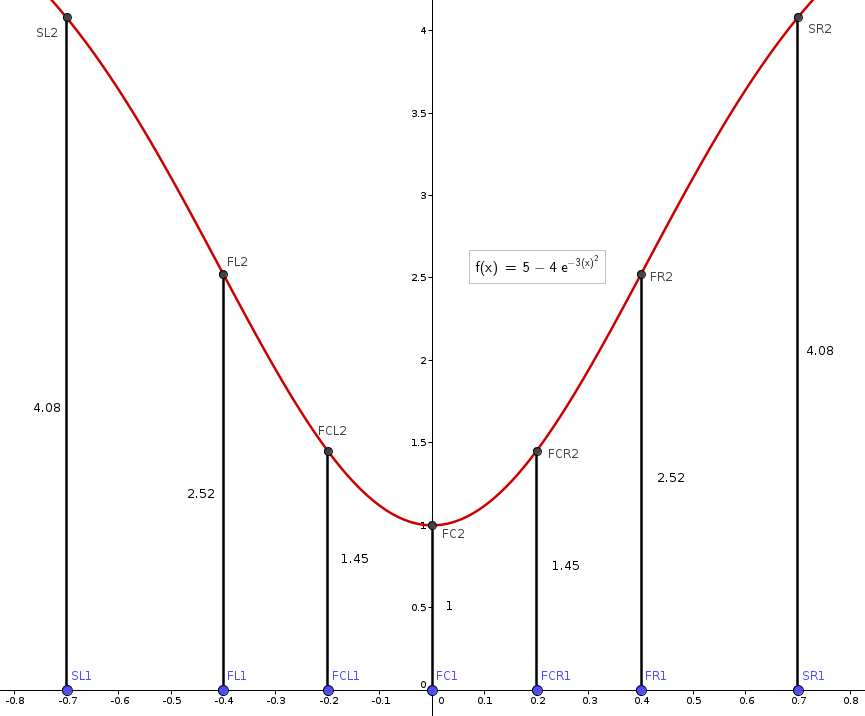
\includegraphics[width=\textwidth, height=11cm, keepaspectratio]{Bilder/Gauss_Sensorgewichtung_gerade.png}
	\caption{Gewichtung der Abstands-Messwerte beim Geradeaus-Fahren}
	\label{img:gaussian-weighted-dist-straight}
\end{figure}

\begin{figure}[ht]
	\centering
	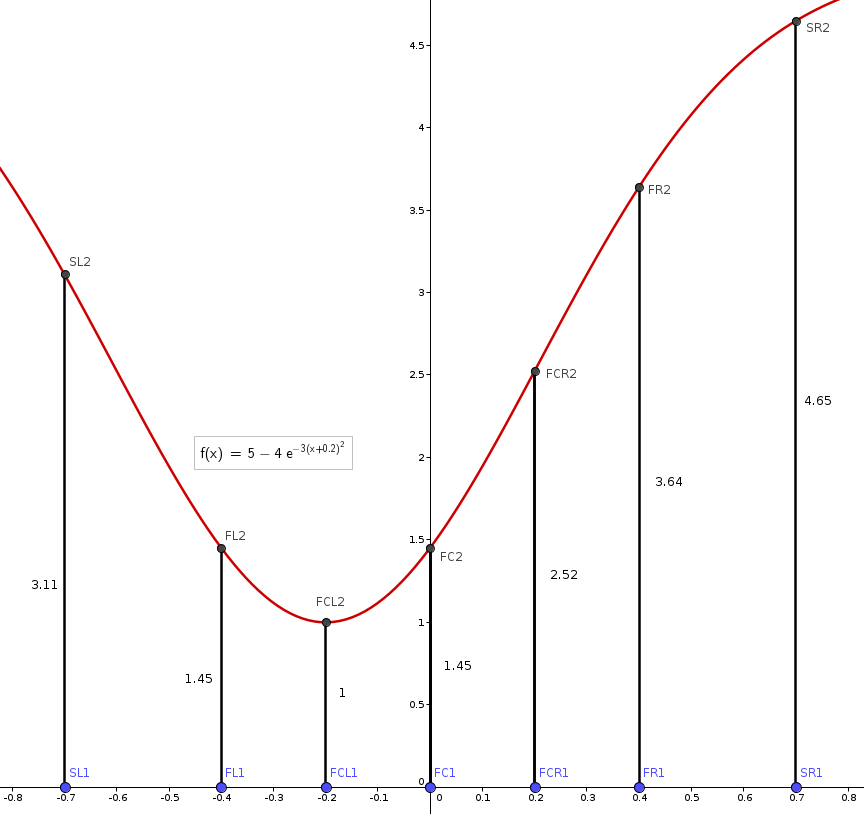
\includegraphics[width=\textwidth, height=12cm, keepaspectratio]{Bilder/Gauss_Sensorgewichtung_geneigt.png}
	\caption{Gewichtung der Abstands-Messwerte bei Lenkung nach links (maximale Verschiebung)}
	\label{img:gaussian-weighted-dist-curve}
\end{figure}

Konkret sieht man in \autoref{img:gaussian-weighted-dist-straight} und \ref{img:gaussian-weighted-dist-curve} die fixen Ablesepunkte der einzelnen Sensoren auf der x-Achse, welche den Sensor-Winkeln in Blickrichtung des Autos angelehnt wurden. Der entsprechende Punkt auf der Gauss-Kurve gibt den jeweiligen Gewichtungs-Faktor an, wobei ein größerer Wert eine größere Unempfindlichkeit bedeutet. Gemäß Lenkwinkel wird nun die Kurve auf der x-Achse verschoben, wodurch die Gewichtung sich auf die entsprechend seitlich liegenden Sensoren verschiebt.

Die Gauss-Kurve entspricht folgender Formel,

\begin{equation}\label{eq:gaussian-weighted-dist}
sensorWeight= 5 - 4 * \exp\Bigl({-3 * (sensorAngle - steeringAngle)^2}\Bigr)
\end{equation}
wobei $sensorAngle$ der auf den Bereich zwischen -1 und 1 normierte Sensorwinkel ist, für den man eine Gewichtung berechnen möchte, und $steeringAngle$ der eingeschlagene Lenkwinkel, ebenfalls im Bereich zwischen -1 und 1 liegend. Die Höhe der Kurve, bestimmt durch die addierte 5 sowie die multiplizierte -4, wurden durch Versuche als angemessen herausgestellt und festgelegt.


\subsubsection{Motoransteuerung}
Die Hauptaufgabe der Motorsteuerung ist das Reagieren auf Flags, wie beispielsweise das Emergencybreak-Flag, sowie das Weitersenden der Motorsteuerungsdaten  an die Arduinokommunikation, welche sie von dem Controller bekommt.

Wir haben uns entschlossen in diesem Baustein auf Flags zu reagieren, um eine schnellere Reaktion auf kritische Ereignisse, wie zum Beispiel das plötzliche Auftauchen eines Hindernisses zu ermöglichen. Dies erreichen wir, indem wir die Flags direkt aus den Blöcken bekommen, welche die Sensordaten verarbeiten und das Signal nicht erst verschiedene Verarbeitungsschritte durchgehen muss. Die Emergencybreak wird erst wieder aufgehoben, sobald ein entsprechendes Signal von den Sensoren kommt.

Außerdem beherrscht dieser Baustein als einziger das Protokoll, welches zur Ansteuerung der Motoren mittels der Arduinokommunication verwendet wird. So kann intern ein Protokoll verwendet werden, das sich deutlich besser lesen und im Falle von Verarbeitungsfehlern debuggen lässt. In diesem Protokoll sehen wir vor, dass die Geschwindigkeit als Prozentwert der Maximalgeschwindigkeit gesendet wird. Dieser wird dann, bestimmt durch Tests, auf den Bereich bis \[\frac{10}{12}\] der maximalen Motorgeschwindigkeit umgerechnet, wobei intern die maximal mögliche Geschwindigkeit mit -12 gegeben ist. Da der Motorcontroller eine gewisse Anzahl an Nullen benötigt, um aktiviert zu werden, werden die ersten 150 Geschwindigkeitsdaten auf Null gesetzt. Nach diesen 150 Nullen können dann Geschwindigkeiten an die Motoren gesendet werden.


\subsubsection{Interprozesskommunikation}

Da die Programmierung in verschiedenen Funktionsblöcken erfolgte, musste eine einheitliche Kommunikation sichergestellt werden. Hierzu wurde eine separate Funktionssammlung erstellt, die von allen Funktionsblöcken inkludiert wurde. Sie beinhaltet Definitionen über den Nachrichtentyp und die Zusammensetzung strukturierter Datentypen. Da der vom ADTF gestellte Ablauf zum Senden oder Empfangen eines bestimmten Nachrichtentyps zur Codeverdopplung in den Funktionsblöcken führen würde, wurden die Funktionen zusammengefasst und ausgelagert. Damit ließ sich auch einheitlich sicherstellen, dass Funktionsblöcke beim Empfangen die Nachricht erst Kopierten, bevor deren Inhalt verändert wurde.

\begin{figure}[ht]
	\centering
	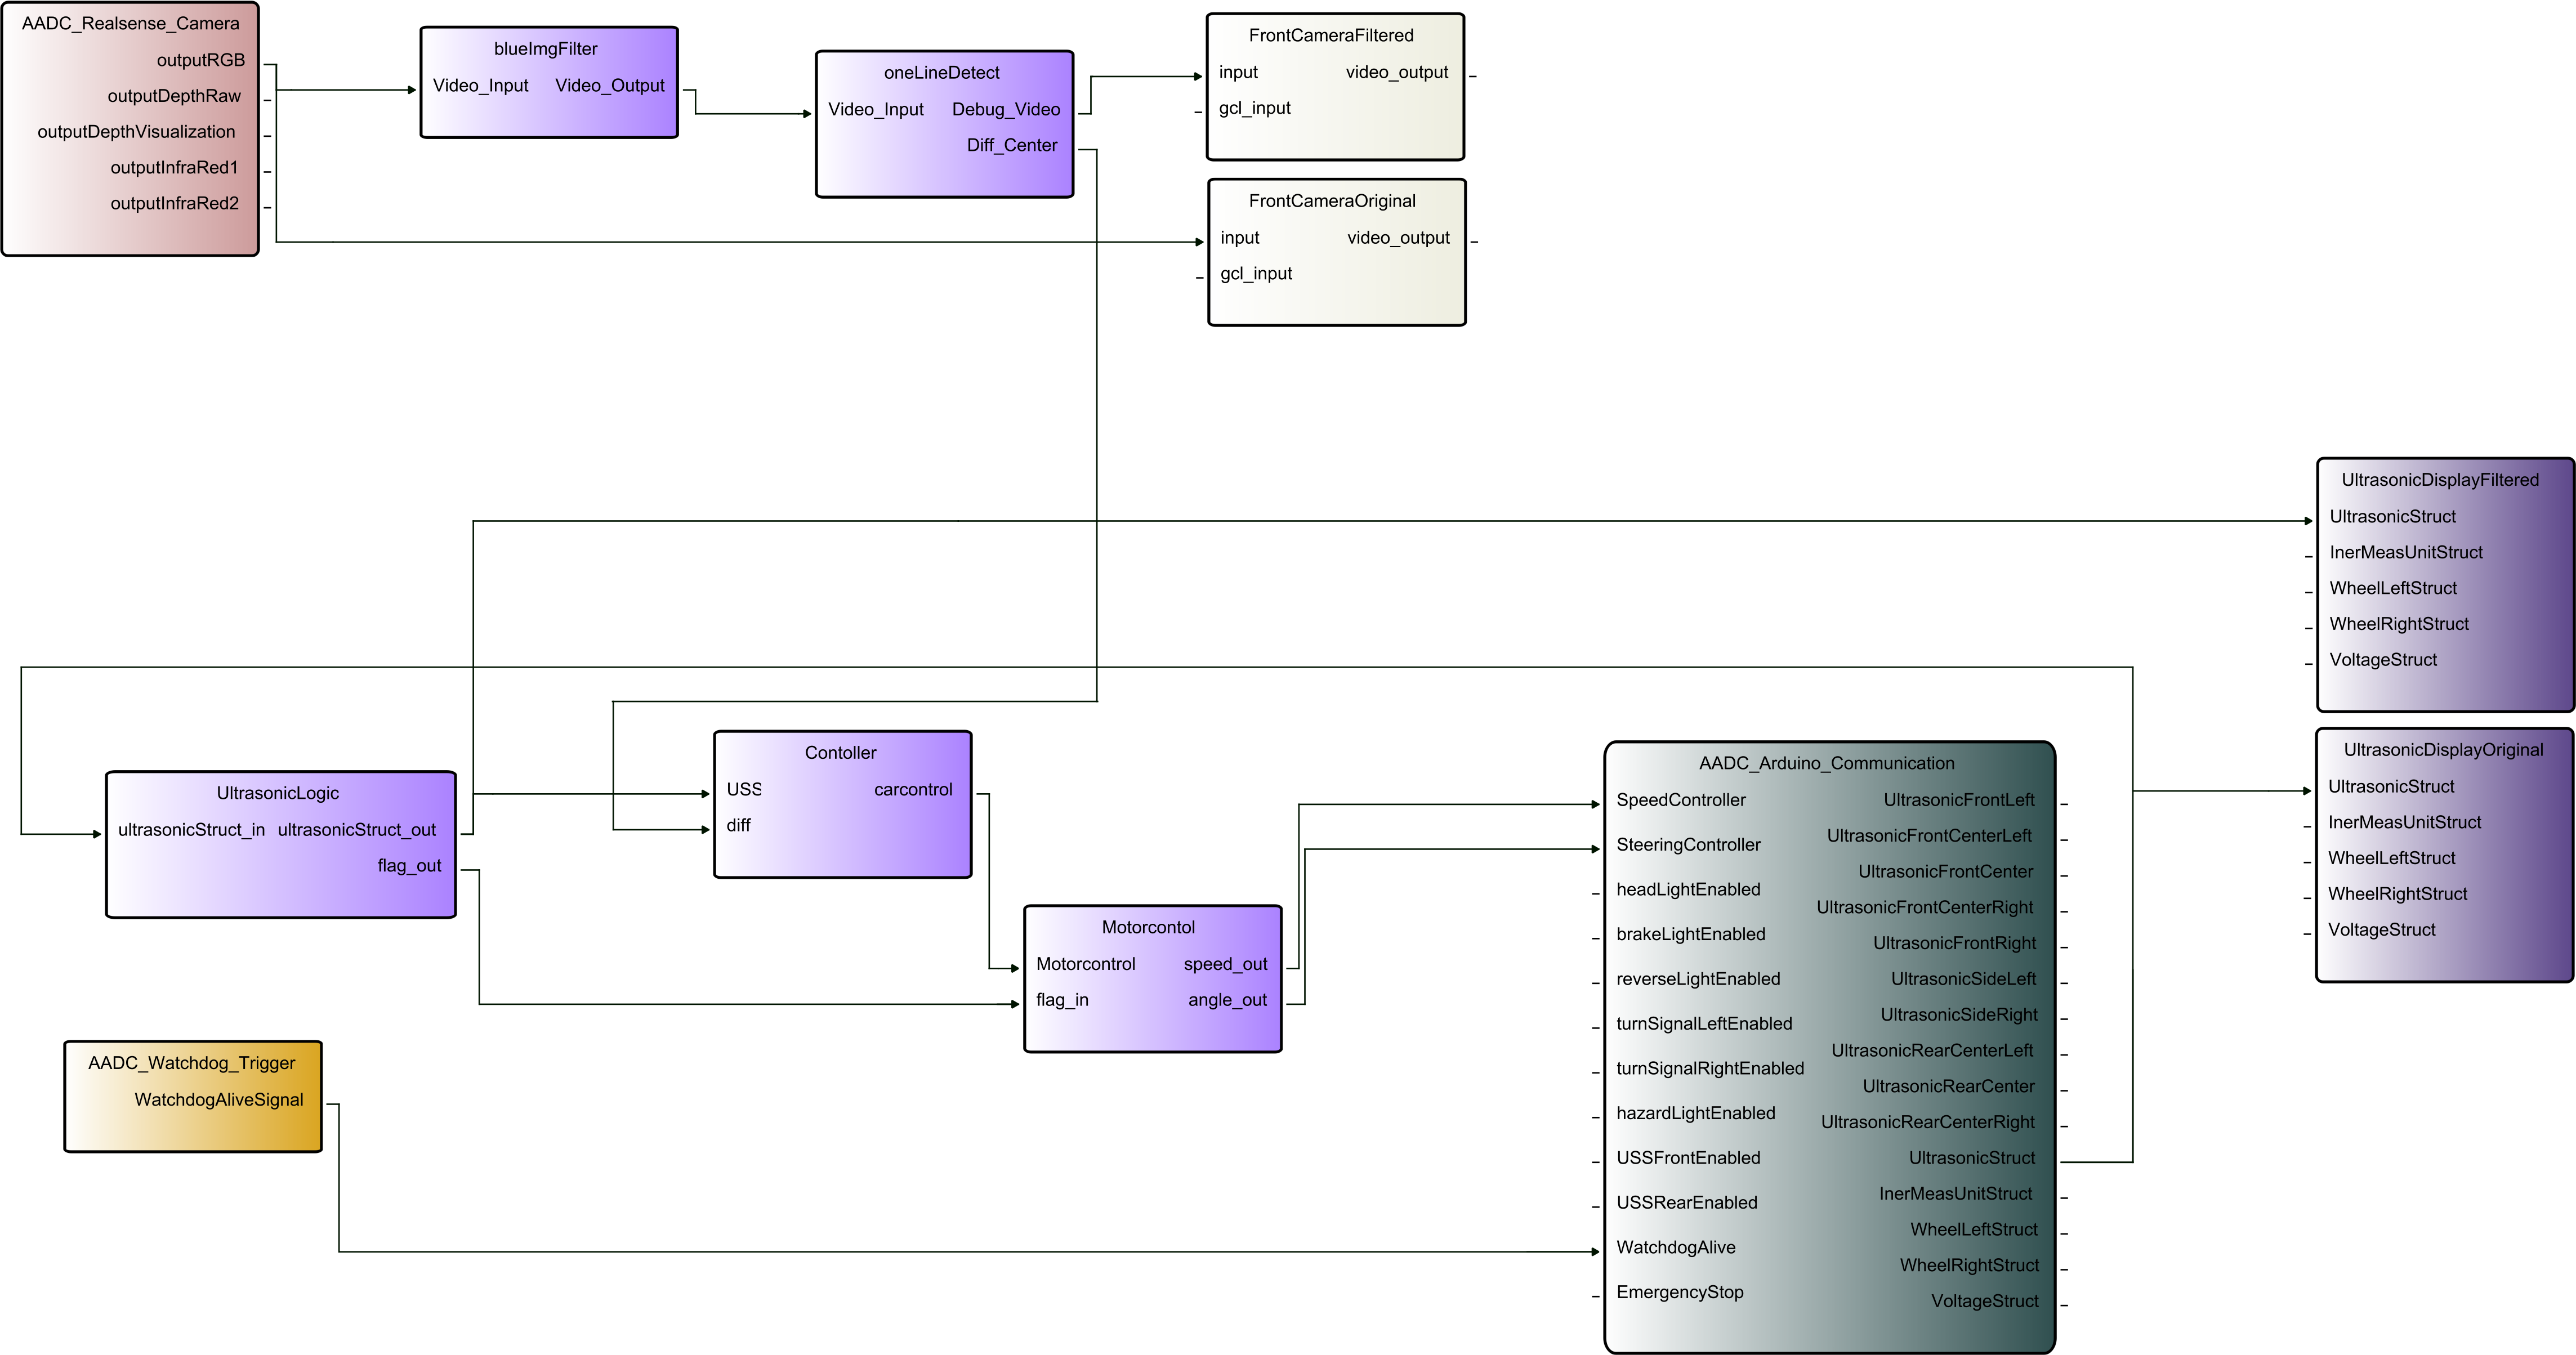
\includegraphics[width=\textwidth, height=\textheight, keepaspectratio]{Bilder/Funktionsblockplan.png}
	\caption{Funktionsblockplan der Test-Umgebung}
	\label{img:funktionsblockplan}
\end{figure}


\subsection{Fallstricke: Komplikationen und Fehler}
Ursprünglich war geplant den Beschleunigungssensor für einen Nothalt zu nutzten, sobald das Auto angehoben wurde. Dies haben wir dann aber nicht implementiert, das es mehrere Probleme mit der Position des Sensors gibt. So wie er momentan verbaut ist, kann man schon Werte von über 2 G (nach Oben) messen, wenn man zum Beispiel den Motor zu schnell beschleunigt, oder abbremst.

\newpage
%%% Neues Kapitel %%%
\section{Auswertung}


\begin{comment}
\newpage
%%% Neues Kapitel %%%
\section{Literaturverzeichnis}

\begin{enumerate}
	\item Im$^2$C Geschichte,  https://www.i2c-bus.org/twi-bus/
	\item Das Im$^2$C-Bus-System
	\item http://www.g-heinrichs.de/pdv/i2c.pdf
	\item http://www.robot-electronics.co.uk/i2c-tutorial
	\item http://www.atmel.com/Images/8183S.pdf
\end{enumerate}
\end{comment}


\newpage
\addcontentsline{toc}{section}{Abbildungsverzeichnis}
\listoffigures

\newpage
\addcontentsline{toc}{section}{Literaturverzeichnis}
\begin{thebibliography}{9}
	\bibitem{aadc-website}
	\textit{AADC-Website},
	Audi AG:
	\url{https://www.audi-autonomous-driving-cup.com/wettbewerb/ueberblick/}
	
	\bibitem{adtf-website}
	\textit{ADTF-Website},
	Elektrobit:
	\url{https://www.elektrobit.com/products/eb-assist/adtf/}
	
\end{thebibliography}

\begin{comment}
\newpage
%\nocite{*}
\cite{aadc-website}
\cite{im2c-bussystem}
\cite{im2c-geschichte}
\addcontentsline{toc}{section}{Literaturverzeichnis}
\bibliography{Dateien/bibliography}
\bibliographystyle{ieeetr}
%\printbibliography
\end{comment}


\begin{comment}
\newpage
\addcontentsline{toc}{section}{Tabellenverzeichnis}
\listoftables

\newpage
\addcontentsline{toc}{section}{Listings-Verzeichnis}
\renewcommand\lstlistlistingname{Listings-Verzeichnis (Quellcode)}
\lstlistoflistings
\end{comment}


\end{document}
